\documentclass[twoside]{book}
\usepackage[top=1in,bottom=1.25in,left=1.25in,right=1in,paperwidth=8in,paperheight=10in]{geometry}
\usepackage{titlesec}
\usepackage{graphicx}

\titleformat{\chapter}[display]{\normalfont\huge\bfseries}{}{0pt}{\Huge}
\titlespacing*{\chapter} {0pt}{20pt}{40pt}

\titleformat{\section}[display]{\center\normalfont\huge\bfseries}{}{0pt}{\huge}
\titlespacing*{\section} {0pt}{20pt}{40pt}

\usepackage{fancyhdr}

\renewcommand{\sectionmark}[1]{\markright{#1}}

\pagestyle{fancy}
\fancyhead{}
\fancyhead[RE,LO]{\thepage}
\fancyhead[RO, LE]{\rightmark}

\fancyfoot{}
\usepackage{blindtext}

\begin{document}

\begin{titlepage}

	\begin{center}
		\vspace*{14em}
		{\Huge A Cookbook of Family Recipes }

		\vspace{3em}
		by

		\vspace{3em}
		{\Large Mona Bridgen}
	\end{center}

\end{titlepage}

\setcounter{page}{1}
\cleardoublepage

\section*{Introduction}
\blindtext

\tableofcontents{}

\chapter{Cakes}
\blindtext
\newpage

	\section{Cake 1}
	\begin{tabular}{p{.5\textwidth} r}
		\begin{itemize}
			\item 2 cup of Flour
			\item 1/2 cup of Sugar
			\item 1/2 cup of Chocolate Chips
			\item 2 Egg
			\item 1/2 cup of sugar
		\end{itemize}
		& \raisebox{-\totalheight}{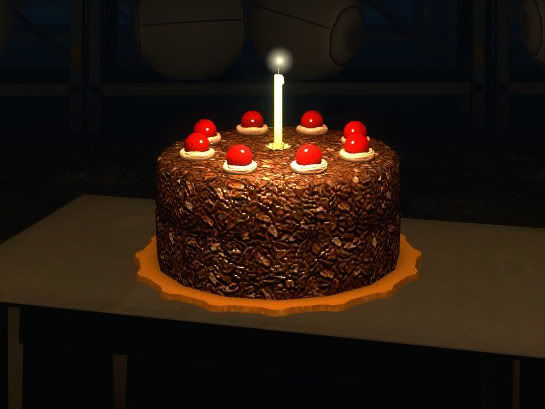
\includegraphics[width=.4\textwidth]{cake.jpg}}\\
	\end{tabular}
	\vspace{5em} 
	\vspace{3em} \hrule
	\vspace{3em} \hrule
	\vspace{3em} \hrule
	\vspace{3em} \hrule
	\vspace{3em} \hrule
	\newpage

	\section{Cake 2}
	\blindtext
	\newpage

	\section{Cake 3}
	\blindtext
	\newpage
\end{document}
